% @author wuTongShuang
% twuac@ust.hk
\documentclass[12pt,a4paper,titlepage]{article}
\usepackage[left=1in,right=1in,top=1.5in,bottom=1.5in]{geometry}
\usepackage{amsthm, amsmath, amsfonts, amssymb, hyperref}
\usepackage{enumerate}
\usepackage{latexsym}
\usepackage{amssymb}
\usepackage{amstext}
\usepackage{fancyhdr}
\usepackage{graphicx}
\usepackage[toc,page,title,titletoc,header]{appendix}
\usepackage{color}
\usepackage{titlesec}
\usepackage{lastpage}
\usepackage{algorithm}  
\usepackage{algorithmic}
\usepackage{caption}
\usepackage{listings}
\usepackage{subcaption}
\usepackage{tikz,mathpazo}
\usetikzlibrary{shapes.geometric, arrows}
\usepackage{tikz}
\graphicspath{{figures/}}
\setlength{\parskip}{7.5pt plus 2pt minus 2pt}

\pagestyle{fancy} 
\lhead{Team \# 39925} 
\rhead{Page \thepage\ of \pageref{LastPage}} 

\setlength{\parindent}{0pt}
\begin{document}

\title{ HICD Model: \\Eradication of Ebola in Ten Days}
\author{\vspace{25pt}\\Team \# 39925\\ \vspace{25pt}}
\date{COMAP Mathematical Contest in Modeling\\February 09, 2015}
\maketitle

\definecolor{ref}{rgb}{1,0,0}
\definecolor{add}{rgb}{1,0,1}

%%%%%%%%%%%%%%%%%%%%%%%%%%%%%%%%%%%%%%%%%%%%%%%%%%%%%%%%%%%%%%%%%
\begin{abstract}
This paper analyzes optimizing the eradication of Ebola infection. We develop a HICD model to explain interactive dynamical system of Ebola infection and the new medication breakthrough. A marginal utility of medicine (MUM) principle for the distribution decision is adopted to minimize the total number of death in the Ebola elimination process. Optimal delivery strategies are proposed for both the medicine distributor located overseas and that located domestically. The result of computer simulation shows that the EVD can be controlled within 10 days, the minimum death is stable at 520 people and the optimal daily production of medicine is around 6000 units per day.
\end{abstract}
%%%%%%%%%%%%%%%%%%%%%%%%%%%%%%%%%%%%%%%%%%%%%%%%%%%%%%%%%%%%%%%%%
\newpage\tableofcontents\newpage

\section{Introduction}

The Ebola virus causes an acute, serious illness which is often fatal if untreated. The current outbreak in West Africa is the largest and most complex Ebola outbreak since the Ebola virus was first discovered in 1976. There have been more cases and deaths in this outbreak than all others combined. Among all the countries influenced, currently the virus concentrates on three of the states, namely Guinea, Liberia and Sierra Leone. However, the World Medication Association has announced a new medication to cure those whose disease are not so advanced, which gives a chance to control and eradicate Ebola from this district. How to set up the manufacturing and logistics system to maximize the effect of the medicine is of great significance. 

In this paper we have taken these factors taken into account:

\begin{itemize}
  \item The spread of the disease
  \item The quantity of the medicine needed
  \item Possible feasible delivery systems
  \item Locations of delivery
  \item Speed of manufacturing of the medicine
  \item Location(s) of manufacturing of the medicine
\end{itemize}

The rest of the report runs as the follows: Section \ref{section_probSet} analyzes the problem and make assumptions for the model,  Section \ref{section_designModel} describes the model for the problem. We then discuss its implementation and experiment results in Section \ref{section_experiment}, and conclude our work in Section \ref{section_conclude}. The Non-Technical Letter is attached after Section \ref{section_conclude}.

\section{Problem Setup}
\label{section_probSet}

The new medicine is a blessing for the general infected but can do nothing to help the patients whose disease is advanced. We approach this problem by grouping a given population of a certain area into 4 categories: 
\begin{itemize}
	\item \textbf{Healthy $(H)$}: those who are susceptible to Ebola, but have not yet been infected and therefore not infectious
	\item \textbf{Infected $(I)$}: those who are currently suffering from Ebola and therefore infectious, but can be cured and become healthy with the newly invented medicine 
	\item \textbf{Cureless $(C)$}: those whose Ebola virus is too advanced to be cured even by the cutting-edge medicine, at the same time they are still alive yet infectious 
	\item \textbf{Death $(D)$}: those who are killed by Ebola and no longer infectious 
\end{itemize}

Our obstacle is that given a fixed speed of manufacturing, medicine is a scarce resource in a limited number of provision per day, hence it is impossible for us to cover every patient in need in a single day. At the same time, Ebola grows at varying rates in different districts with distinct size of initial infection population, so we have to decide a priority of medicine distribution, aiming at saving infected people as much as possible from getting advanced to the status of the cureless. According to WHO Ebola Situation Report \cite{ebolaReport20140204}, the most severely affected countries are \emph{Guinea}, \emph{Sierra Leone} and \emph{Liberia}. There are totally 61 districts in these three countries. Our job is to design an optimal strategy of distributing the medicine to the 61 stricken districts so as to minimize the total number of death within the possibly shortest time span. Moreover, with the possibly lowest death achieved, we wish the delivery cost and medicine production cost can be kept to a minimum in our delivery system.


In this paper, we make the following general assumptions, so as to balance its level of generality and reality:
\begin{enumerate} [D. 1]
	\item As long as a patient takes 1 unit of medicine, he will be healthy in the next period. However, he is still susceptible to Ebola as all other healthy people.
	\item During a typical day, an infected patient will have the opportunity to take the medicine (if there is any) before being determined whether he is cureless or not. 
	\item The medicine is not proactive and only effective for the infected, that is to say, a healthy person only takes medicine after he gets infected. 
	\item We assume that the entire population, $N=H+I+C+D$, is a constant. Therefore, there is no birth rate in any district, and thus horizontal disease transmission is the only possible form. 
	\item Population mobility among different districts is prohibited.
\end{enumerate}

First, we create a plane mechanics model to solve the three portions. Next we establish a computer model to solve the three portions better. What's more, we have evaluated the influence of the sweet spot makes, and also solved why the corked bat and the aluminum bat are prohibited.

\tikzstyle{startstop} = [rectangle, rounded corners, minimum width=3cm, minimum height=1cm,text centered, draw=black]
\tikzstyle{io} = [trapezium, trapezium left angle=70, trapezium right angle=110, minimum width=3cm, minimum height=1cm, text centered, draw=black]
\tikzstyle{process} = [rectangle, minimum width=3cm, minimum height=1cm, text centered, draw=black]
\tikzstyle{decision} = [diamond, minimum width=3cm, minimum height=1cm, text centered, draw=black]
\tikzstyle{arrow} = [thick,->,>=stealth]

\section{Design of the Model}
\label{section_designModel}
The overall workflows is as the follows:
\begin{center}
\begin{tikzpicture}[node distance=2cm]
 %定义流程图具体形状
\node (start) [startstop] {Start};
\node (in1) [io, below of=start] {Load Data};
\node (pro1) [process, below of=in1] {Fit $v$};
\node (pro2) [process, below of=pro1] {Determine destination};
\node (pro3) [process, below of=pro2] {Determine delivery strategy};
\node (pro4) [process, below of=pro3] {Applying nedicine for destination};
\node (pro5) [process, below of=pro4] {Applying Ebola evolving matrix};

\node (dec1) [decision, right of=pro5, xshift=3.5cm] {$\forall I_n,C_n = 0$?};
\node (pro6) [startstop, below of=dec1, yshift=-1cm] {End};

 %连接具体形状
\draw [arrow](start) -- (in1);
\draw [arrow](in1) -- (pro1);
\draw [arrow](pro1) -- (pro2);
\draw [arrow](pro2) -- (pro3);
\draw [arrow](pro3) -- (pro4);
\draw [arrow](pro4) -- (pro5);
\draw [arrow](pro5) -- (dec1);


\draw [arrow](dec1) -- node[anchor=east] {yes} (pro6);
\draw [arrow](dec1) |- node[anchor=south] {no} (pro2);
\end{tikzpicture}
\end{center}
\subsection{The Dynamic System of Ebola Infection}
\label{section_dynamicInfect}
In the epidemiology field, the dynamics of epidemics are often based upon SIR model \cite{kermack1927contribution}, which characterize people into three classes: the susceptible, the infective and the removed. The problems in this model are:
\begin{enumerate}
	\item People can only be infected once. Note that this is over-optimistic about the immunity. For a mysterious disease like Ebola, this may not be true.
	\item SIR does not recognize that there is a fourth category of people whose conditions are so advanced that they have to die, yet unlike the dead, they are still living and thus infectious to healthy people. Indeed, the characterization of the classic SIR model leaves no room for predicting the possible consequence of a new drug trial.
\end{enumerate}

Based upon the four types of people we state in Section \ref{section_probSet}, we design the following discrete-time dynamical system of Ebola infection in the form of a linear system:

\begin{equation}
	\label{eqn_dynamicInfect_basic}
	\begin{cases}
		H_{i, n+1} & =  H_{i,n} - v \cdot (C_{i,n} + I_{i,n})  \\
		I_{i, n+1} & = (1+v-q) \cdot I_{i,n} + v \cdot C_{i,n}  \\
		C_{i, n+1} & = (1-f) \cdot C_{i,n} + q \cdot I_{i,n}  \\
		D_{i, n+1} & =  D_{i,n} + f \cdot C_{i,n}
	\end{cases}
\end{equation}

Here $H_n$ is the cumulative number of healthy people in the period $n$, In is the cumulative number of infected people in the period $n$, $C_n$ is the cumulative number of cureless people in the period $n$, $D_n$ is the cumulative number of death in the period n. In our case of Ebola, the period is daily. $i$ denotes different districts.

As for the parameters, we have:

\begin{itemize}
	\item $v$: the speed of horizontal Ebola transmission, i.e., $v$ healthy people will be infected by 1 patient (no matter he is infected or cureless). Note that $v$ varies both across districts and periods, i.e., $v=f(n,i)$;
	\item $q$ ($\in[0,1]$): the probability that an infected patient whose Ebola virus develops so fast becomes cureless.
\end{itemize}

Upon setting, the Ebola effect is represented by a transformation matrix:
\begin{equation}
	\label{eqn_dynamicInfect_trans}
	\textbf{E} = 
	\begin{bmatrix}
		1 & -v & -v & 0\\
		0 & 1+v-q & v & 0\\
		0 & q & 1-f & 0\\
		0 & 0 & f & 1\\
	\end{bmatrix}
\end{equation}

The population distribution of a district is denoted by a four dimensional vector:
\begin{equation}
	\label{eqn_dynamicInfect_vec}	
	\textbf{X}_{i,n} = 
	\begin{bmatrix}
		H_{i,n} \\
		I_{i,n} \\
		C_{i,n} \\
		D_{i,n} \\
	\end{bmatrix}
\end{equation}

Therefore the dynamical system of Ebola infection can be written as the following matrix format: 
\begin{equation}
	\label{eqn_dynamicInfect_matrix}
	\textbf{X}_{i,n+1} = \textbf{EX}_{i,n}
\end{equation}

Above describes the n-period process without medication.

\subsection{The Dynamical System of Medication}
\label{section_dynamicMedi}

As known, with full medication, the infected population can be cured and thus add themselves into healthy population. However, according to the statement of the problem A, the medicine has no effect on the cureless.

Accordingly, if we give a district full medication (=$I_{i,n}$ units of medicine), we can write a collection of linear equations to describe the medication process:

\begin{equation}
	\label{eqn_dynamicMedi_basic}
	\begin{cases}
		H_{i, n+1} & =  H_{i,n} + p \cdot I_{i,n}  \\
		I_{i, n+1} & = (1-p) \cdot I_{i,n} \\
		C_{i, n+1} & = C_{i,n} \\
		D_{i, n+1} & =  D_{i,n}
	\end{cases}
\end{equation}

The medicine effect can therefore be represented by a transformation matrix 
\begin{equation}
	\label{eqn_dynamicMedi_trans}
	\textbf{M} = 
	\begin{bmatrix}
		1 & p & 0 & 0\\
		0 & 1-p & 0 & 0\\
		0 & 0 & 1 & 0\\
		0 & 0 & 0 & 1\\
	\end{bmatrix}
\end{equation}

Where $0\leq p \leq 1$ denotes the level of preparedness \cite{ebolaPrepare20140204} of a given district. This implies that due to various logistics reasons, not all of the medicine given to a district can be fully utilized by its patients. The parameter $p$ captures the potential waste of the medicine due to management problem and it varies across districts $(p=f(i))$. We include this term to make our model more realistic.

The dynamical system of medication can be written as:
\begin{equation}
	\label{eqn_dynamicInfect_matrix}
	\textbf{x}_{i,n+1} = \textbf{MX}_{i,n}
\end{equation}
As a consequence, a typical day for a district receiving In units of medicine can be written as a matrix equation:

\begin{equation}
	\label{eqn_dynamicInfect_matrix}
	\textbf{x}_{i,n+1} = \textbf{MEX}_{i,n}
\end{equation}

Note that by our assumption, the medication process precedes the Ebola deterioration.
\begin{equation}
    \textbf{ME} = 
         \begin{bmatrix}
             1 & -v+p(1+v-q) & (p-1)v & 0\\
             0 & (1+v-q)(1-p) & (1-p)v & 0\\
             0 & q & 1-f & 0\\
             0 & 0 & f & 1
         \end{bmatrix}
\end{equation},
Therefore, we have
\begin{equation}
    I_{i,n} = (1+v-q)(1-p)\cdot I_{i,n}+(1-p)v\cdot C_{i,n}
\end{equation}
For the medication effect overrides the Ebola infection effect, it follows that
\begin{equation}
    I_{i,n} < I_{i,n}
\end{equation}
Solve the above linear equation w.r.t. $p$: 
 \begin{equation}
    p > 1 - \frac{1}{1-q+(1+C_n/I_n)v}
\end{equation}

In short, we will sort the targeted districts with method introduced in Section \ref{section_MUM}, and we will give a district full medication to the proritized districts, and only stop when the epidemic situation is for sure under control. Here, $C$ and $I$ are used as our constraints. In the cases that our left medicine could not cover a whole district, we will give medicine to a portion of local people. The concrete medicine distribution method is summerized in Algorithm \ref{algm_partition}. 

\begin{algorithm}[h] 
    \caption{Partitioning district vector \textbf{X}$_{i,n}$} 
    \begin{algorithmic}[1]
    \REQUIRE \textbf{E}: infection matrix, \textbf{M}: medicine matrix,\textbf{X}: district matrix, \textbf{numMedi}: number of medicine unit available
    \ENSURE Optimize the impact of medicine distribution
    \STATE Sorting the district for recieving medicine with method introduced in Section \ref{section_MUM}
    \WHILE{\emph{I and C are all zero}}
        \IF {$I_{i,n} < numMedi$}
            \STATE /*Split \textbf{X}$_{i,n}$ as a linear combination of two vectors*/
            \begin{eqnarray*}
            \textbf{X}_{i,n} &\gets & \textbf{X}_{i,n}^{(1)} + \textbf{X}_{i,n}^{(2)}
                             \begin{bmatrix}
                                        H_{i,n}\\ I_{i,n}^{(1)}\\ C_{i,n}\\ D_{i,n}
                                     \end{bmatrix}
                                     +
                                     \begin{bmatrix}
                                        0\\ I_{i,n}^{(2)}\\ 0\\ 0
                                     \end{bmatrix},\\
            I_{i,n}^{(1)}  & \gets &  n\\
            distributedMedicine &\gets &numMedi
            \end{eqnarray*}   
        \ELSE
            \STATE \begin{equation*}
                     \textbf{X}_{i,n}^{(1)} \gets \textbf{MX}_{i,n}, \textbf{X}_{i,n}^{(2)} \gets zeroVector, distributedMedicine \gets numMedi
                    \end{equation*}
        \ENDIF
        \begin{eqnarray*}
            \textbf{X}_{i,n}^{(1)'} & \gets & \textbf{MX}_{i,n}^{(1)}\\
            \textbf{X}_{i,n+1}^{(1)'} & \gets & \textbf{E}(\textbf{X}_{i,n}^{(1)'} + \textbf{X}_{i,n}^{(2)})
        \end{eqnarray*}
    \STATE $numMedi \gets numMedi + distributedMedicine + productedMedicine$
    \ENDWHILE
        \label{algm_partition}

\end{algorithmic} 
\end{algorithm}

\subsection{Distribution Priority Determination}
\label{section_MUM}
In our model, one of the most important step is to determine which districts could get the medicine first. Our primary concern is the number of death. Mathematically, the goal of optimization is to minimize $\sum{D}$. The problem we are facing is that at the original stage demand for medicine per day exceeds its daily supply. A priority rule of distributing medicine has to be designed.

For any given district $i$ in any given period $n$, we can calculate the efficiency of an incremental unit of medicine (equivalently, marginal utility of medicine ``MUM''):
\begin{eqnarray}
    I_{i,n+1} - I_{i,n} & = & (v-q)I_{n}+vC_{n}\\
    MUM & = & \frac{\partial(I_{i,n+1}-I_{i,n})}{\partial(I_{i,n})}\\
        & = & v-q
\end{eqnarray}

We will rank $v-q$ from highest to lowest and send medicine starting from the highest until all the medicines are used up. The intuition behind is that the larger $v-q$ is, the more patients one additional unit of medicine can save. In this way, we are maximizing the utility of the medicine and therefore minimizing the number of death because we serve the districts with the most urgent need.

Let $\mu$ denotes the daily production of medicine, which is a constant in our model. 
Given any period $n$, Assume $v_{1,n}< v_{2,n}< v_{3,n}<...< v_{j-1,n} < v_{j,n}<...< v_{61,n} (1 \leq j \leq 61)$, if it satisfies
\begin{equation}
	\label{eqn_dynamicInfect_basic}
	\begin{cases}
		\sum_{k=j}^{i}I_{k, n} & \leq \mu  \\
		\sum_{k=j-1}^{61}I_{k, n} & > \mu  \\
	\end{cases}
\end{equation}
$I_{i,n}$ units of medicine will be delivered to district $i$ for $i=j,j+1,j+2,...,61$. The medicine left, namely, $\mu-\sum_{i=j}^{i=61}{I_{i,n}}$ will go to district $j-1$:
\begin{itemize}
    \item For districts $i=j,j+1,j+2,...,61$, they will follow the matrix transformation of the full medication,
    \item For district $j-1$, it will follow the matrix transformation of the partial medication,
    \item For districts $i=1,2,...,j-2$, they will follow the matrix transformation of Ebola alone.
\end{itemize}

\begin{figure}[htbp]
    \centering
    \label{img_vfit}
    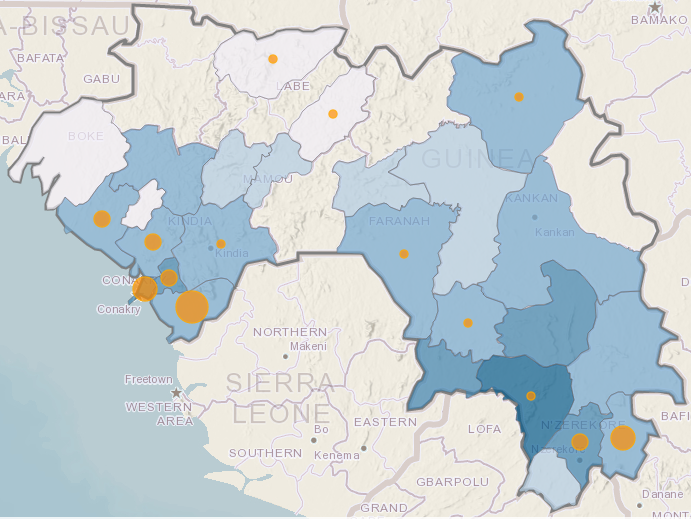
\includegraphics[width=0.6\textwidth]{figures/imgSpreadMapG.png}
    \caption{Distribution map of GUINEA from $WHO$, with saturability of blue representing population, size of orange circle representing the severeness of epidemic situation
.}
\end{figure}




\section{Medicine Delivery Strategy}

In the last section we have theoretically established a lower bound of number of death and a minimum of total medicine production, and have shown that these can be obtained by our MUM priority rule. Our next concern should be how we can deliver the medicine in accordance with our priority list in an economically efficient way, in other words, minimize the transportation costs.

Apart from locations of delivery, the location of the medicine distributor is a crucial factor for our analysis of the most feasible delivery system design. Since there lack some information about where the medicine is intended to be produced, in this section, we propose two possible locations of the medicine distributor: One single overseas distributor in US, where the medicine is most likely being created and patented, or multiple African laboratory distributors in Guinea (which is the only member country among the three) together with the respective delivery strategy. Due to the expensive transportation fee, we do not consider third party member country. Also, due to the fact that  the rule for sharing medical patented items are very strict and could take too long to proceed, we do not consider other possible production parties.

The model is explained below.

\subsection{Single Overseas Distributor Model (SOD Model)}

In this model, it's assumed that the World Medical Association located at US is the single overseas distributor of the medicine. WMA is thus exclusively responsible for the delivery to the 61 districts in West Africa. The medicine is directly shipped from US to various destinations in West Africa. 

West Africa is a compact region and thus compared to the overseas shipping distance, inland transfer within Africa is relatively minimal, therefore we further assume that the medicine shipped to one district can be directly transferred to its adjacent districts within the same day with no additional cost. However, the transfer can only take place once. 

\begin{figure}[htb]
\centering
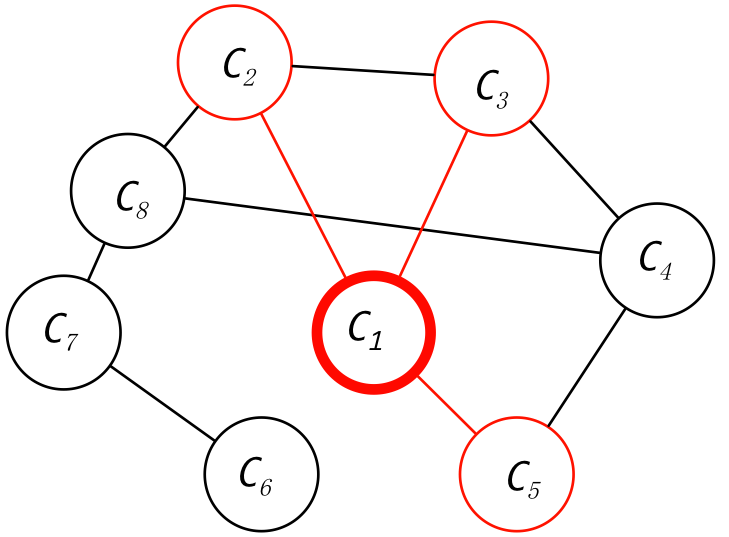
\includegraphics[width=0.4\textwidth]{figures/imgSingleModelMap.png}
\caption{\label{MultiDemo}Deliver arrangement of Single Overseas Distributor Model}
\end{figure}

The deliver strategy can be illustrated by the “model1Map”. For instance, $C_1$ is adjacent to $C_2$, $C_3$ and $C_5$. If we find that we need to send medicine to both $C_2$ and $C_5$ based upon the MUM priority rule but it is costly to deliver twice, then our best strategy is to give the total demand of $C_2$ and $C_5$ to $C_1$ and let the medicine transported to $C_2$ and $C_5$ proportionally afterwards.

By increasing proportion of local transportation, this strategy can help us reduce the times of overseas delivery which largely curtail the transportation expenses.

\subsection{Multiple Domestic Distributors Model (MDD Model)}

Among all the three countries we focus on, only Guinea is a member of World Medicine Association who is licensed to produce WMA's product outside US border. This means the other two countries have to import the medicine from Guinea. In Africa, when a kind of medicine is imported, the medicines have to go through the recipient country's capital and then be distributed to the destinations of the country. 

\begin{figure}[htbp]
\centering
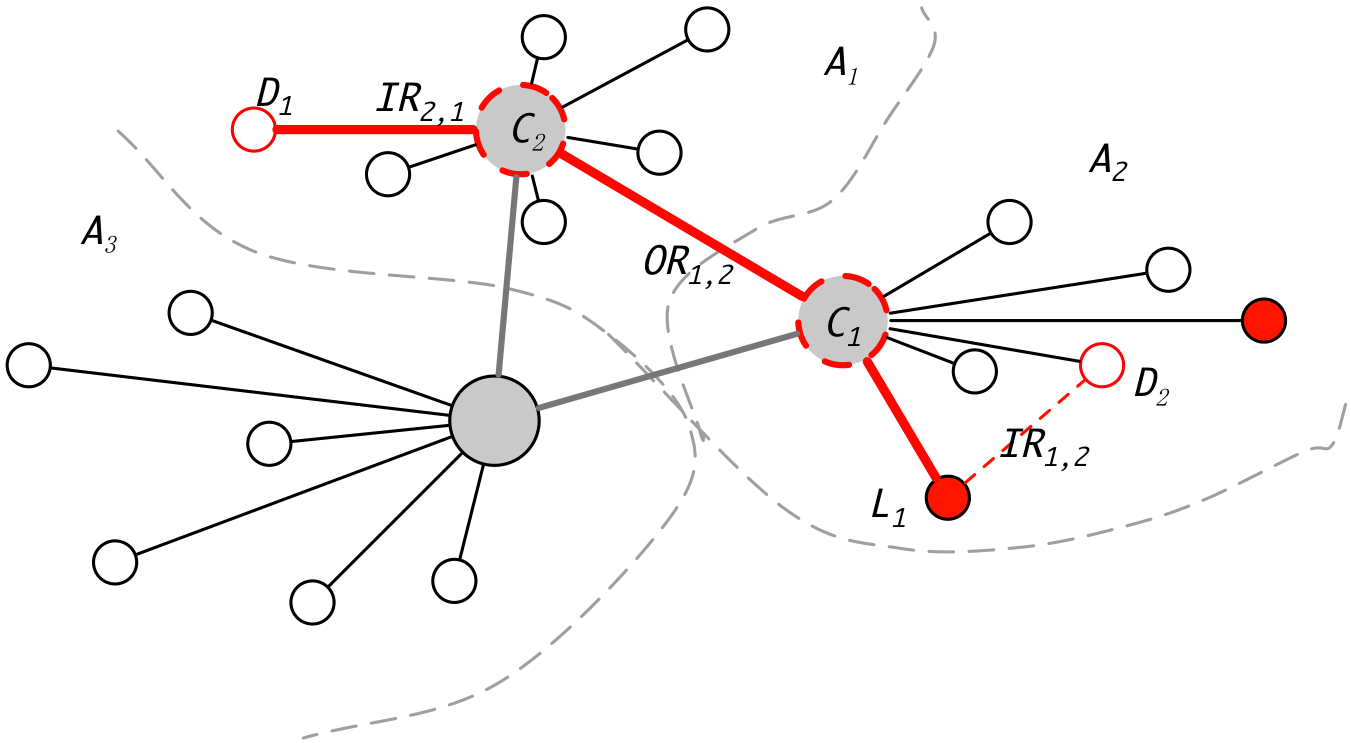
\includegraphics[width=0.6\textwidth]{figures/imgDoubleModelMap.png}
\caption{\label{MultiDemo}Deliver arrangement of Multiple Domestic Distributors Model}
\end{figure}

The deliver arrangement can be illustrated by Figure \ref{MultiDemo}. For instance, $L_1$ is one of the laboratories in $A_2$, $C_1$ and $C_2$ are the capitals of $A_1$ and $A_2$ respectively, $D_1$ and $D_2$ are the districts of $A_1$ and $A_2$ respectively. If $D_2$ demands medicine from $L_1$, the delivery will take the inner route IR$_{1,2}$. If $D_1$ demands medicine from $L_1$, the delivery will go through $C_1$ then $C_2$ and thus take the route $IR_{1,1}+OR_{1,2}+IR_{2,1}$. 

Based upon WHO situation summary report, there are currently five Ebola laboratories in Guinea, and thus these five laboratories are assumed to be the pharmaceutical sites for the whole West Africa.

Each day each laboratory will produce a certain amount of medicine. The distribution policy is that each laboratory will first satisfy the need of the district it belongs to, for convenience and inexpensiveness consideration, and then distribute the remaining medicine to other districts through Simplex Method \cite{simplex1991}.

Simplex Method is a well-known algorithm for linear programming. As a systematic procedure for generating and testing candidate vertex solutions to a program, it has been widely used in logistic models to optimize the point-to-point delivery system, which suits our goal perfectly. It is widely implemented and established throughout the history thanks to its proved usefulness. Because of its reputation, and the fact that our objective could be transformed into a typical linear program intuitively, as long as we express it in the following form:
\begin{eqnarray}
    \text(minimize )   & &f = \textbf{C$^{T}$X} \\
    \textbf{subject to}& & \textbf{Ax}  \leq  \textbf{B}\\
                       & & \textbf{X} \geq 0
\end{eqnarray}

Simplex Method could solve it intuitively.

Since:
\begin{itemize}
    \item our objective is to find an optimized way to allocate the medicine so that the total transportation cost is minimized,
    \item the transportation cost between laboratory i and destination j is calculated as $Cost_{i,j}=n\cdot d$, where $n$ is the number of medicine to be transported, $d$ is the cost associated with each unit of medicine to be transported between $i$ and $j$, and is proportional to the distance between $i$ and $j$. 
\end{itemize}

Therefore, in linear program format shown before, $f$ is the total cost function, $C$ is the transportation cost function, tansportationA is the constrain matrix for linking transportation method \textbf{X}, the demanded medicine amount and the producted medicine amount. The relationship between lab, treatment center anddistrict could be found in \cite{ebolaReport20140204}. In this way, Simplex Method could help with the next step. 


\section{Experiment Results}
\label{section_experiment}

We implemented our model in Matlab, which is famous for data analysis. \footnote{The open source code could be found in Github: https://github.com/leafsherry/MCM2015}
In this section, we first introduce our database and the  the confirmation of variables value in Section \ref{section_database}, And test our models in Section\ref{section_modelTest}.


\subsection{Data information and Variable Confirmation}
\label{section_database}
We choose data from $WHO$ with consideration of its authority and the richness of its database. The data we got includes:
We tested our model with the following data: 
\begin{itemize}
    \item \emph{Time-series data of epidemic situation of Ebola}. with consideration of its authority and the richness of its database. We obtained the up-to-date situatioin changes, from September 2014 to Feb 2015, for all districts \cite{ebolaDatabase20140204} three countries with severe illness, namely \emph{Guinea}, \emph{Sierra Leone} and \emph{Liberia}. This includes the number of newly confirmed or suspected illness cases, number of new death, and number of healthy people per day. 
    \item \emph{Population distribution of all districts}.、\cite{WMADatabase20140204} Note that the data contains a certain level of error, e.g. for some districts where the most current population are not available, it is computed by ourselves with the available population history and the growth rate for timeline consistency.
\end{itemize}



We use these two databases, with some additional knowledges regarding of Ebola, to confirm the values for used variables. Though most of them have been mentioned in Section \ref{section_designModel}, these variables are summerized here for clearness:
\begin{itemize}
    \item \emph{p: preparedness of a given district}. From \cite{WMADatabase20140204}, $p$ is commonly distributed from 0.06 to 0.64. We generate differen p for every district. Since it is a randomly drawn value therefore introduces great uncertainty into our system, We specifically run experiments to confirm its effect in Section \ref{section_3d}.
    \item \emph{v: infection rate}. It is generated as a time based function from WHO data, with the real rate at each day computed as: 
    \begin{equation*}
        R_{n-1} = \frac{\sum \text{newly confirmed or suspected patients in Day $n$}}{\sum \text{confirmed or suspected patients in Day $n-1$}}
    \end{equation*}
    The real data are then curve-fitted to obtain the $v$-function, as shown in Figure \ref{img_vfit}.
    \item \emph{q: probability of becoming curless}. Based on its 2 to 20 days' incubation and the rapidness of the incoming deterioration, we assume it to be 0.1.
    \item \emph{f: probability of death}. It is confirmed in \cite{ebolaInfo20140204} that the average fatality rate is 0.5, and therefore we assign this to $f$.
    \item \emph{$\mu$: Daily production of medicine. }Due to lack of information, we do not try to estimate it, but rather use it to test which number may be appriate.
\end{itemize}


\begin{figure}[htbp]
\centering
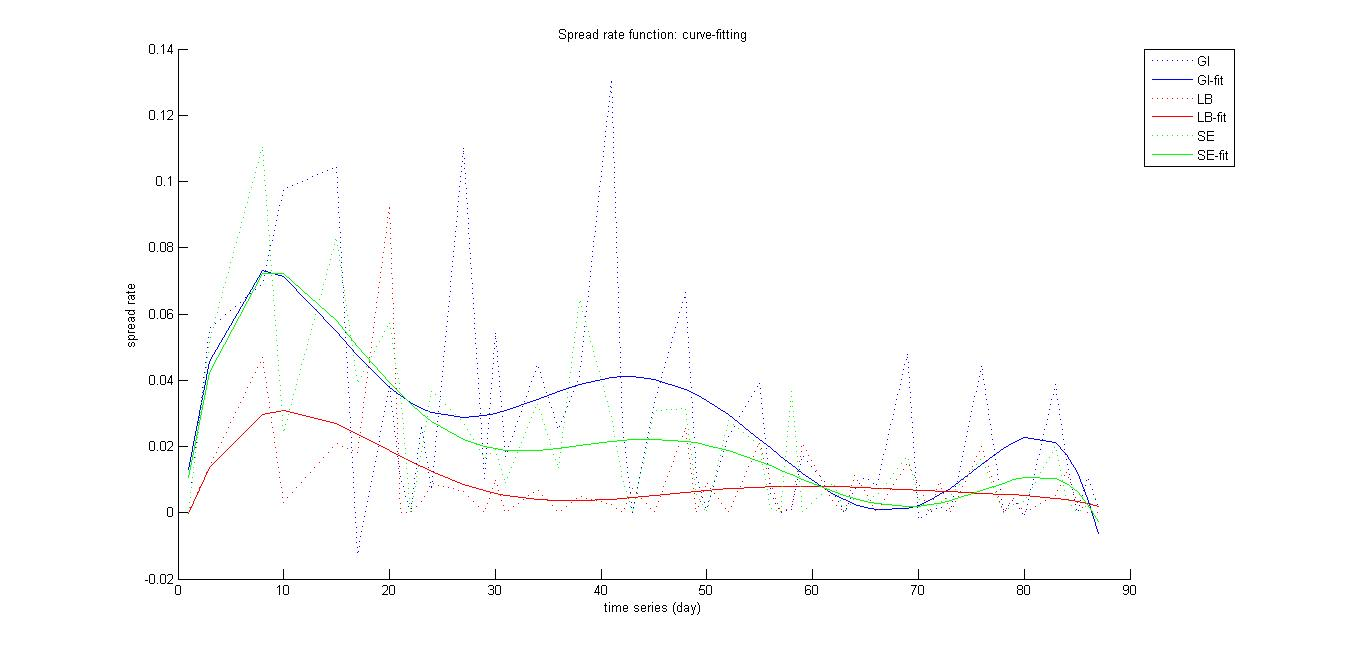
\includegraphics[width=1\textwidth]{figures/imgVfit.jpg}
\caption{\label{vgraph}Polyfit graph of $v$. The dash lines present the time series tendency for the number of cases in $Guinea$, $Sierra Leone$ and $Liberia$. The solid lines show the fitting curve of v for the three countries under HICD model. As can be seen, our model of Ebola infection is realistic and predictive of the disease spreading pattern.}
\label{img_vfit}
\end{figure}

\subsection{Model Comparison}
\label{section_modelTest}

In this part, we intend to compare the two proposed methods in terms of number of days needed to control the situation and the number of total death in the epidemic period, given the same amount of medicine per day.  Here, the total population of the three countries is summed to be of ten thousands, and our daily medicine production $\mu$ is set to be varying up to the population, so as to discuss the best solution. We first build the baseline in Section \ref{model_baseline}. We present the results individually, in Section \ref{section_testSingleModel} and Section \ref{section_testMultiModel}, and then discuss the differences in Section \ref{section_compareModel}.

\subsubsection{Testing Without Giving Medicine}
\label{model_baseline}
A testing run without medicine distribution is ignited inspired by the negative value of calculated p, which indicates that the epidemic is actually receding. The result shows that the epidemic will end after 90 days and the number of death is around 560. The effect of the medicine is to decrease the number of deaths and the time needed to end this epidemic. The declining of the epidemic is also shown in real-life data given by $WHO$, from which the $v$ used in this paper is derived.

\subsubsection{Single Overseas Distributor Model (SOD Model)}
\label{section_testSingleModel}

\begin{figure}[htbp]
  	\centering
  	\begin{subfigure}[b]{1\textwidth}
      	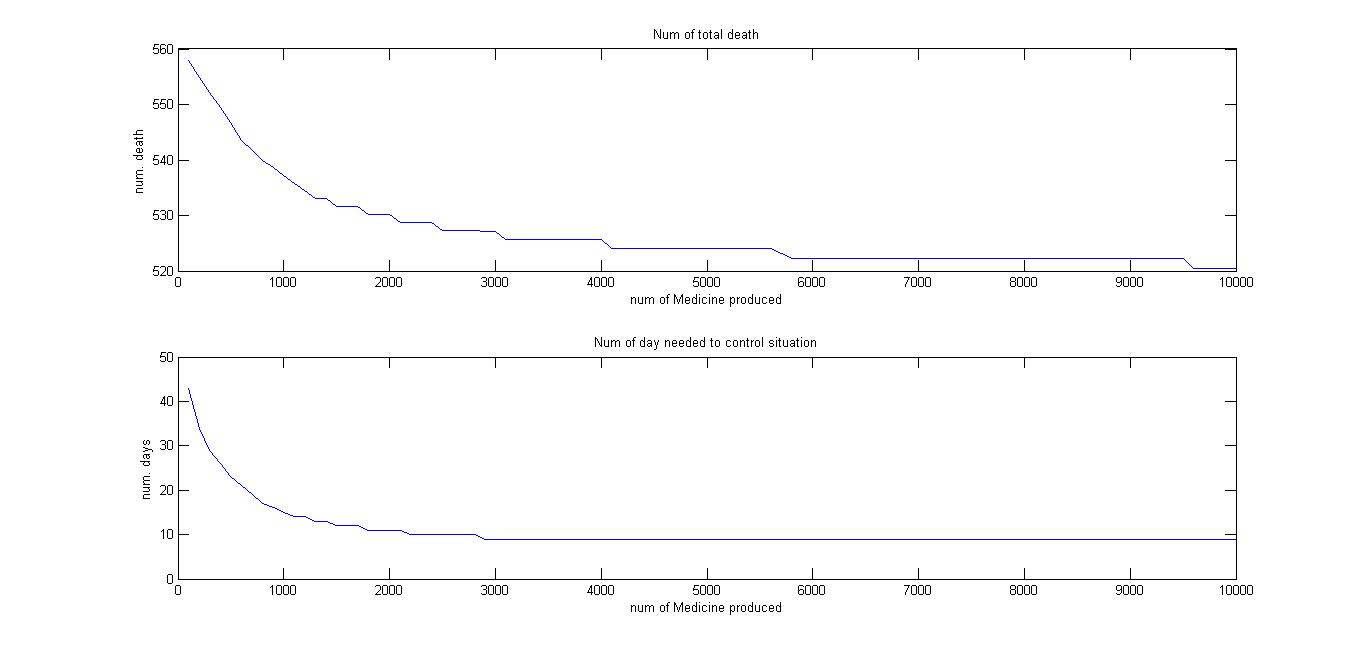
\includegraphics[width=\textwidth]{figures/imgSingleShort.jpg}
      	\label{figure_singleModel_short}
      	\caption{Result for SOD Model, $\mu \in [0, 10000]$}
  	\end{subfigure}
  	\begin{subfigure}[b]{1\textwidth}
      	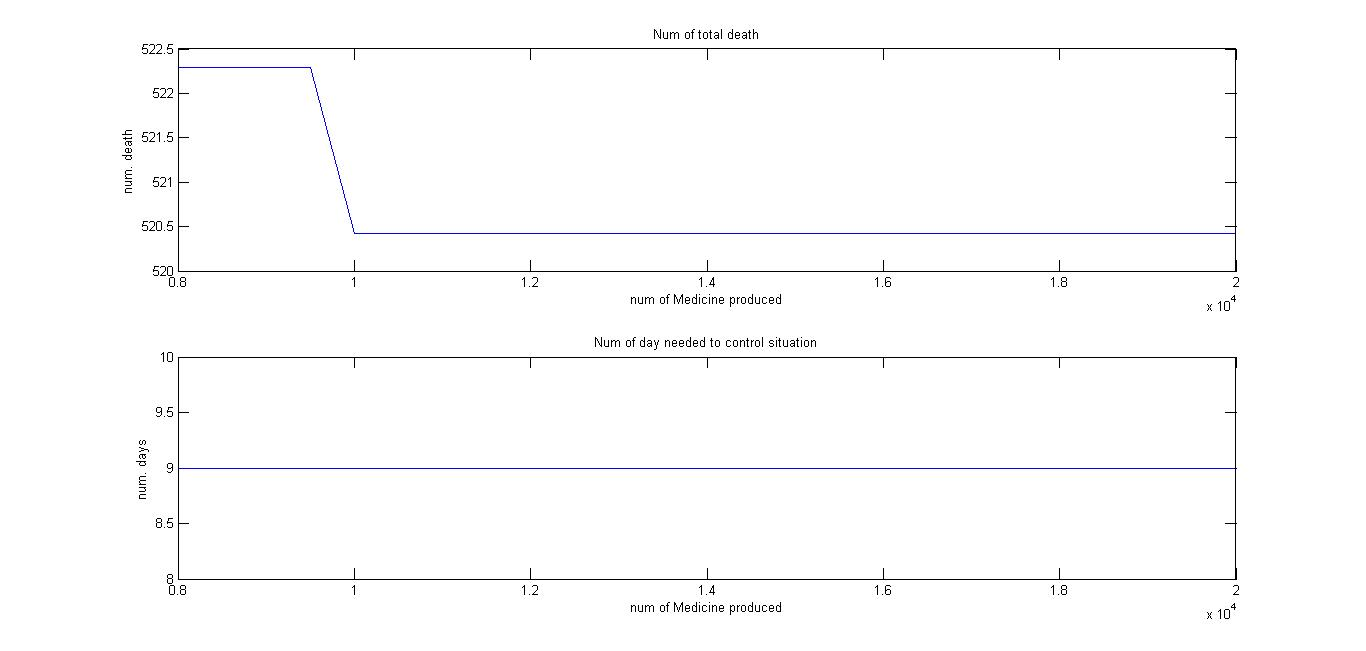
\includegraphics[width=\textwidth]{figures/imgSingleLong.jpg}
   		 \label{figure_singleModel_long}
   		 \caption{Result for SOD Model, $\mu \in [8000, 20000]$}
  	\end{subfigure}
  	\caption{The total death and number of days needed to eliminate Ebola with respect to the daily production of medicine under Single Overseas Distributor model.}
  	\label{figure_singleModel}
\end{figure}

\begin{figure}[htbp]
  	\centering
  	\begin{subfigure}[b]{1\textwidth}
      	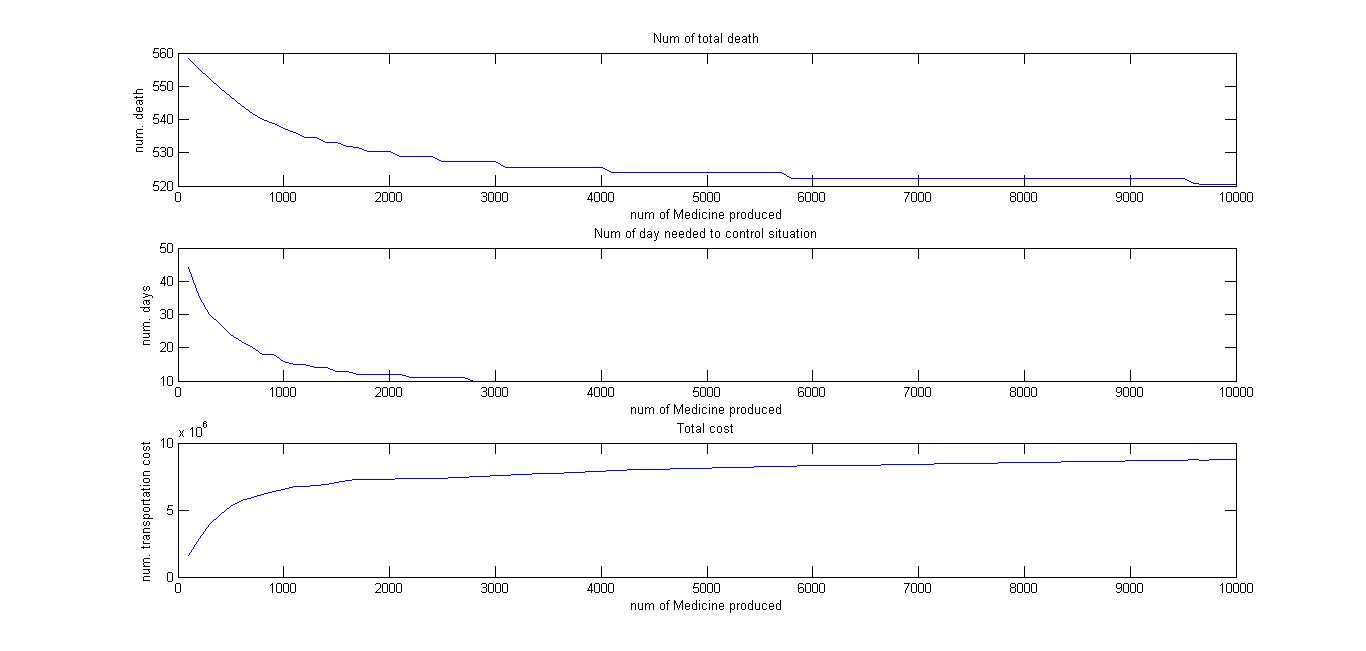
\includegraphics[width=\textwidth]{figures/imgMultiShort.jpg}
      	\label{figure_multiModel_short}
      	\caption{Result for MDD Model, $\mu \in [0, 10000]$}
  	\end{subfigure}
  	\begin{subfigure}[b]{1\textwidth}
      	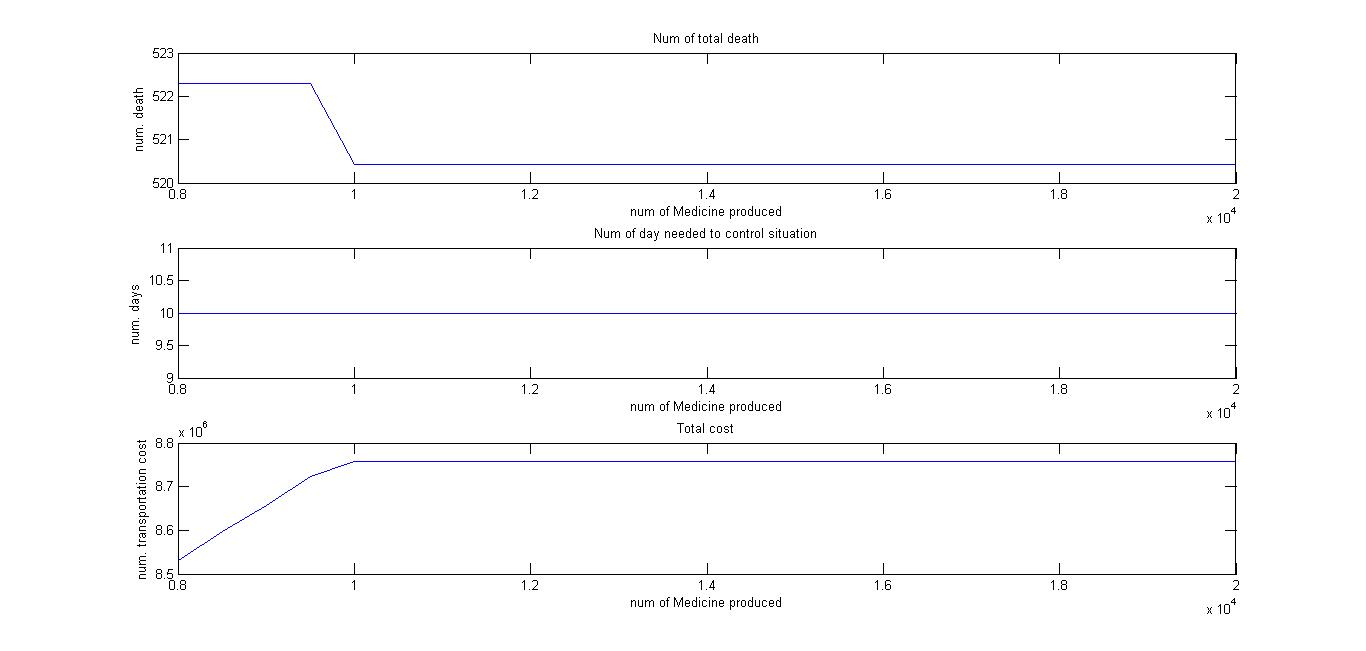
\includegraphics[width=\textwidth]{figures/imgMultiLong.jpg}
   		 \label{figure_multiModel_long}
   		 \caption{Result for MDD Model, $\mu \in [8000, 20000]$}
  	\end{subfigure}
  	\caption{\label{MultiDomDis}The first two plots give the total death and number of days needed for elimination and the third plot gives the total delivery cost with respect to the daily production of medicine under Multiple Domestic Distributors model.}
  	\label{figure_multiModel}
\end{figure}


Figure \ref{figure_singleModel} shows The experiment result. Since the great varies of the obtained values with respect to $\mu$, we separate the line graph into two sub-line graphs, each shows approximate half of the who $\mu$ range. The minimum value is determined by running the model in a larger range of medicine productivity. From the graph, we can see that both the number of death and the number of days needed decrease and decrease more slowly as the productivity of medicine increases. The minimal duration needed to eliminate Ebola is 9 days and the minimum death is 520. The graph also suggests that an optimal productivity should be around 6000 per day.

Note that, since comparing to the transportation expense for US, local transporation fee could be dismissed, we do not count it into our result.

\subsubsection{Multiple Domestic Distributors Model (MDD Model)}
\label{section_testMultiModel}

Figure \ref{figure_multiModel} has similar settings as Figure \ref{figure_singleModel}, except for having on more sub-graph, namely the transportation cost. The first two curves show the same trend is similar to the result of MOD Model, whereas the minimum time needed is 10 days and the minimum death is 520. The increment in the minimum time makes sense because the strategy used here is that each laboratory satisfies the need of its own district at first, therefore violating the strategy of MUM priority principle, which will decrease the efficiency, thus adds the minimum time. The cost increases as the pharmaceutical productivity increases, which implies that the manufacturing rate should be kept as efficient as possible when the requirements of number of deaths and number of days needed are met. A reasonable value of productivity suggested in the figure is also around 6000.

\subsubsection{Comparison Between Two Models}
\label{section_compareModel}
The fundamental difference between these two models is where the production of medicine takes place. In this certain circumstance, the difference between the efficiency of the two models is not so obvious, in the sense that the minimum numbers of death and the best value of productivity are the same and the minimum numbers of days differ only by 1. Therefore considering total budget, it is suggested that the medicine be produced in Guinea, in a sense that air transportation is much more expensive than land transportation.

\subsection{3D Graphics: Eliminating p's uncertainty}
\label{section_3d}

\begin{figure}[htbp]
  	\centering
  	\begin{subfigure}[b]{0.45\textwidth}
      	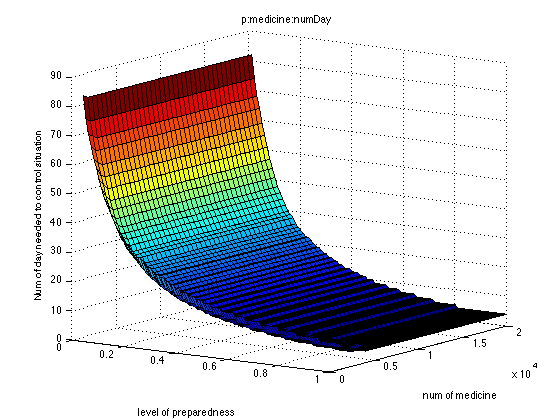
\includegraphics[width=\textwidth]{figures/imgpMedDay1.png}
      	\label{figure_3dDay1}
      	\caption{3D for Day}
  	\end{subfigure}
  	\begin{subfigure}[b]{0.45\textwidth}
      	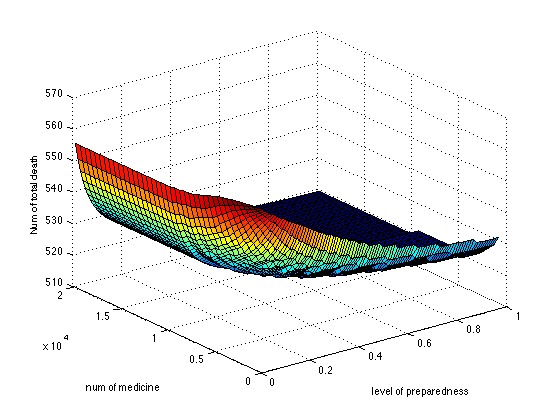
\includegraphics[width=\textwidth]{figures/imgpMedDeath1.png}
      	\label{figure_3dDeath1}
      	\caption{3D for Death}
  	\end{subfigure}
  	\begin{subfigure}[b]{0.45\textwidth}
      	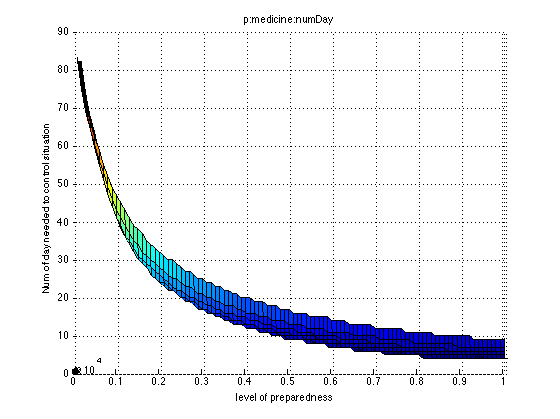
\includegraphics[width=\textwidth]{figures/imgpMedDay2.png}
      	\label{figure_3dDay2}
      	\caption{3D for Day}
  	\end{subfigure}
  	\begin{subfigure}[b]{0.45\textwidth}
      	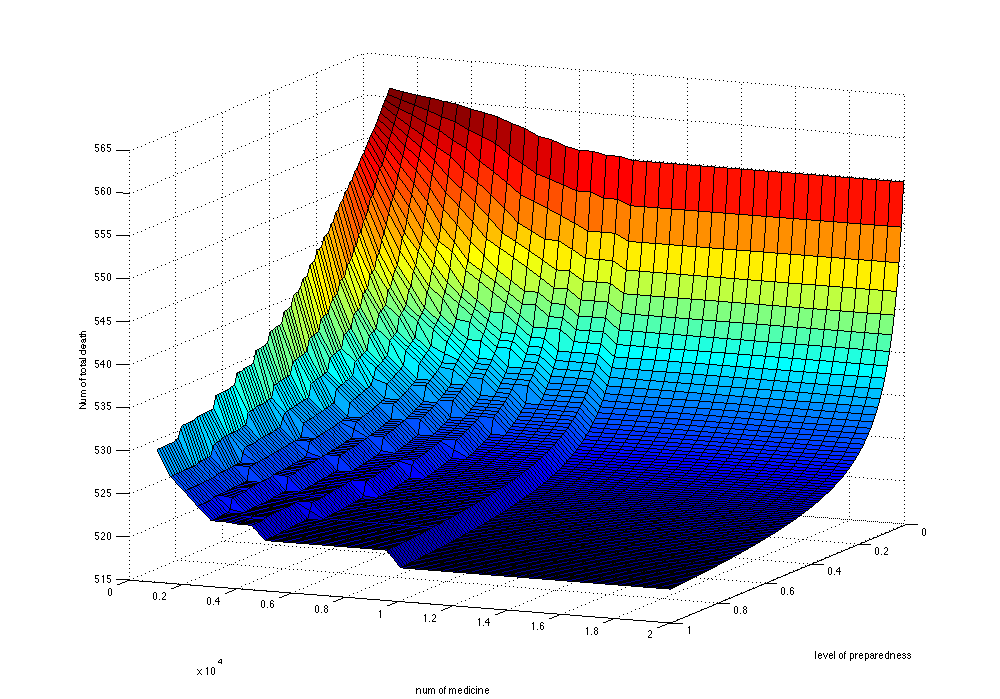
\includegraphics[width=\textwidth]{figures/imgpMedDeath2.png}
      	\label{figure_3dDeath2}
      	\caption{3D for Death}
  	\end{subfigure}
  	\begin{subfigure}[b]{0.45\textwidth}
      	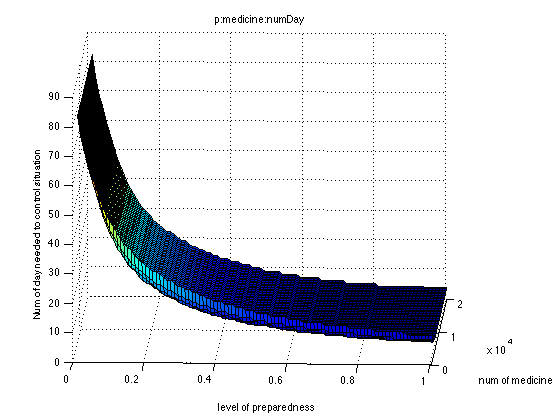
\includegraphics[width=\textwidth]{figures/imgpMedDay3.png}
      	\label{figure_3dDay3}
      	\caption{3D for Day}
  	\end{subfigure}
  	\begin{subfigure}[b]{0.45\textwidth}
      	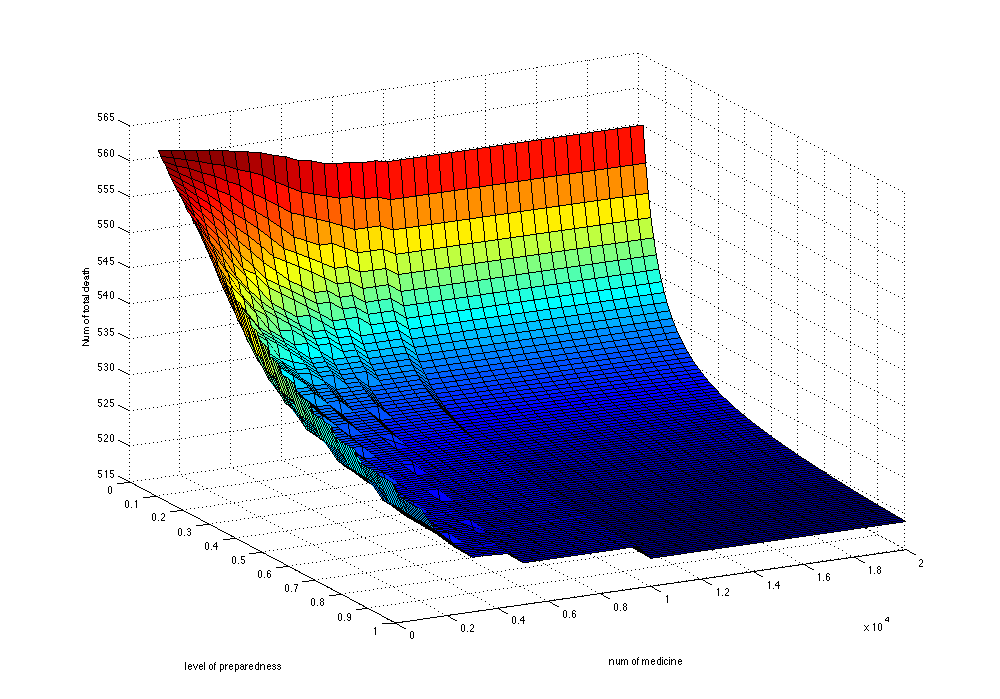
\includegraphics[width=\textwidth]{figures/imgpMedDeath3.png}
      	\label{figure_3dDeath3}
      	\caption{3D for Death}
  	\end{subfigure}
  	\caption{3D model generated with $p$ and $\mu$ as independent variable. The three on the left are different view points for modeling the days needed to eliminate Ebola, while those on the right for the number of total death.}
  	\label{figure_3d}
\end{figure}



As mentioned before, $p$, the preparedness of a given district, is generated different p for every district. Since it is a randomly drawn value therefore introduces great uncertainty into our system, We specifically run experiments to confirm its effect by including it as an independent variable using together with $\mu$. The results are as following. 


In Figure \ref{figure_3d}, the left three figures displays the dynamics of the days needed to eliminate Ebola subject to the value of p and the daily production of the medicine. It is observed that the number of days decreases as p and productivity increases, and that if $p=0$ or no medicine is given, the epidemic will end itself within 90 days. The figure also shows that when p is small, it will significantly lengthen the duration of elimination. This has policy implications that countries at risk should make good management and surveillance to fight the disease.

The right three figures displays the dynamics of the total death subject to the value of p and the daily production of the medicine. The trend is similar as that of the previous plot, but not as sharp. In this graph, p also plays a significantly negative role when its value is small. If $p=0$ or no medicine is given, the epidemic will end itself with around 565 fatalities.


\section{Conclusion}
\label{section_conclude}
This paper presents a four-dimensional model, namely HICD model, to explain the interactive dynamical system of Ebola infection and the new medication implementation, which is beyond the scope of the classic SIR model in the epidemiology field. By the construction of the HICD model, the Ebola problem becomes an initial value problem of first-order difference equations. The solution of the linear system shows that there is a minimum requirement for p (preparedness) to make the effect of the new medication superior to the Ebola devastating effect. 
Regarding how to distribute the new medicine, we designed a principle of marginal utility of medicine (MUM). This principle can guarantee us to maximize the utility of the medicine and therefore minimize the number of potential death.
The choice of the best delivery strategy depends on the location of the medicine distributor. If the World Medicine Association acts as the single overseas distributor, transportation can be reasonably curtailed by sending the medicine to adjacent districts. If there are multiple African laboratory distributors in Guinea, simplex algorithm is adopted for the optimization of the transportation costs by transforming the delivery system into a typical linear program.
The result of computer simulation using current WHO data and statistics shows that the EVD can be controlled within 10 days, the minimum death is stable at 520 people and the optimal daily production of medicine is around 6000 units per day. We further explore the negative relationship between preparedness and number of death.
The strength of model lies upon its creative insights and completeness. For example, the classic SIR model leaves no room for predicting the possible consequence of a new drug trial. In contrast, by differentiating the cureless from the traditional “removed” category, our HICD model can make validated prediction for the future Ebola trend affected by the new medication on a more realistic basis. Furthermore, we take all the possibilities into account, especially with regard to the location of the medicine distributor, and come up with optimal delivery strategy for each possible location.
The limitations of our model could be time lag for the Ebola virus to take effect, such as the incubation period. This limitation might be solved by formulating higher order difference equations.


\newpage
\section{Non-Technical Letter}

On behalf of the World Medical Association, in light of the severe situation of Ebola virus in West Africa, I am proud to announce that we have found a new medication which could cure Ebola and help African people to a great extent. It brings hope to those who still live under the fear of this horrible disease, especially the countries of Guinea, Liberia, and Sierra Leone. Based on the fact that these three countries suffer the most from the epidemic, we have investigated the situation of these countries and have projected a delivery strategy to make the best use of the medicine.

The strategy we developed can minimize the fatality caused by the EVD from now on and will also end the epidemic as soon as possible. The disease could be eradicated from West Africa within 10 days if the level of preparedness is met. The total death could be reduced to 520. To achieve these, the manufacturing speed of medicine should be at least 6000 units per day, which is a reasonable amount within our ability. 

We would give priority to those districts with the most urgent need and would try in due diligence to save the patients if possible. Whether or not we would be able to set up laboratories in Africa to produce the medicine does not really make difference in the effective control of Ebola according to our research based on current statistics, but the transportation budget can be curtailed a lot if we would be able to produce it inside Africa. Therefore we would try our best to set up production inside Guinea, which is the only member state of WMA among the three severely influenced countries. 

Apart from our arrangement, the coordination of countries are equally important, since our research shows that if not all the medicine could be fully utilized, the number of total death and the duration could be doubled or even tripled. This is why we are calling upon our fellow countries Guinea, Liberia and Sierra Leone to improve their epidemiological surveillance, case management and responsiveness which their own people can benefit the most from.

We have also found out yet another piece of good news. According to contemporary data, even if no medicine would be used, the epidemic will end in around 3 months. Therefore there should be no fear for an endless epidemic to cause countless casualties. However if the medicine is used we can save 80 days and lots of lives. Since life is invaluable and time is priceless, we strongly urge the related parties to implement the new medication according in accordance with this announcement. 

We do hope that the new medication could bring a downturn to Ebola threat our globe is facing. For the sake of mankind, we hereby call upon national and local governments, international humanity organizations and anyone who cares about his/her miserable fellows suffering in West Africa to join hands, to fight Ebola and win this war!
%%%%%%%%%%%%%%%%%%%%%%%%%%%%%%%%%%%%%%%%%%%%%%%%%%%%%%%%%%%%%%%%%
\newpage
\begin{thebibliography}{99}

\bibitem{ebolaReport20140204} World Health Organization, ``Ebola Situation Report - 4 February 2015",\\http://paws.kettering.edu/~drussell/bats-new/sweetspot.html,February 9th, 2015.
%1
\bibitem{kermack1927contribution} Kermack, W. O., \& McKendrick, A. G. (1927, August). A contribution to the mathematical theory of epidemics. In Proceedings of the Royal Society of London A: Mathematical, Physical and Engineering Sciences (Vol. 115, No. 772, pp. 700-721). The Royal Society.
%2
\bibitem{ebolaPrepare20140204} World Health Organization, ``Preparedness Indicators",\\http://apps.who.int/ebola/en/current-situation/preparedness-indicators, February 9th, 2015.

\bibitem{ebolaDatabase20140204} World Health Organization, ``Ebola data and statistics",\\http://apps.who.int/gho/data/node.ebola-sitrep.quick-downloads?lang=en February 9th, 2015.

\bibitem{WMADatabase20140204} WMA, ``Members' List",\\http://www.wma.net/en/60about/10members/21memberlist/index.html February 9th, 2015.

\bibitem{simplex1991} Stone, R. E., \& Tovey, C. A. (1991). The simplex and projective scaling algorithms as iteratively reweighted least squares methods. SIAM review, 33(2), 220-237.

\bibitem{ebolaInfo20140204} World Health Organization, ``Ebola virus disease",\\http://www.who.int/mediacentre/factsheets/fs103/en/ February 9th, 2015.


\end{thebibliography}

\end{document}

